\chapter{模型简介}
\label{chap:machine-learning-models}

同一批已标注邮件，可以支持几种不同的预测办法。我们可以学习特征权重，也可以逐层执行条件规则，还可以保存旧邮件，在预测时查找相近记录。第\ref{chap:introduction}章只选择了第一种形式，并用训练确定其中的参数。本章要进一步说明：这些形式各自保存了什么关系，比较它们时应该考察哪些对象。

两个分类器可能给出相同标签，却采用不同表示。一个保留固定权重，另一个依靠历史实例；一个直接计算得分，另一个还描述类别概率。因此，我们分别考察表示规模、变量的概率语义、关系形式、输出接口，以及损失和学习准则。这五项描述模型及其学习设定的不同方面，其中损失连接任务评价与模型选择，不属于预测函数本身。第一卷的函数空间、概率推断、范数与评分规则在这里用于解释比较依据。我们先建立模型族、具体模型与训练的区别，再把分类和聚类放到同一组维度中比较。

\section{什么是模型}
\label{sec:models-meaning}

在第\ref{chap:introduction}章的邮件例子中，输入仍是$\bm{x}=(x_1,x_2)^{\top}$，两个分量分别表示促销词次数和链接数。规定加权求和后计算垃圾邮件概率，只确定了一种形式。权重不同，同一输入的概率也可能不同，因此训练前面对的是一组候选关系，训练后才选出实际使用的一项。满足给定形式与约束的候选集合称为\term{模型族}（model family），记为$\mathcal H$；一个具体模型记为$h\in\mathcal H$。预测任务也常把这个集合称为假设空间。“模型族”还可以用于描述聚类、降维与分布建模的候选对象。

候选范围确定之后，还要填入使模型可计算的信息。邮件分类要确定特征权重，聚类可能要确定中心，数据压缩可能要确定投影方向。它们的对象不同，都在把模型族中的可能形式变成一个具体模型。

在选定表示下，由数据估计并用来确定具体模型的量称为模型参数。回归系数、中心坐标和网络权重都具有这项作用。我们用$\bm{\theta}$记录这些量，$h_{\bm{\theta}}$表示相应的具体模型。

为直接对照单个函数与候选集合，我们沿用邮件参数$\bm{\theta}=(b,w_1,w_2)^{\top}$，写成
\begin{equation}
  \begin{aligned}
    h_{\bm{\theta}}(\bm{x})
      &=\frac{1}{1+\exp[-(b+w_1x_1+w_2x_2)]},\\
    \mathcal{H}&=\{h_{\bm{\theta}}:\bm{\theta}\in\mathbb{R}^{3}\}.
  \end{aligned}
  \label{eq:models-family-example}
\end{equation}
其中，$w_1,w_2$是两个特征的权重，$b$是在加权和之外加入的偏置。
集合$\mathcal{H}$包含所有允许的权重组合所确定的模型；例如，令
$b=-2$、$w_1=0.8$、$w_2=0.3$，就选出了其中一个具体模型。
这些数值是概念示例。换参数仍在同一集合内选择，换成条件分支树则改了候选关系的形式，属于另一模型族。

模型族还没有给出怎样作出选择。学习算法读取数据并调整参数，例如邮件算法根据训练样本更新三个数。更换优化步骤，可以保持同一个候选范围，却得到不同的选择过程或结果。因此，模型族说明可选对象，参数值及其模型说明选定对象，学习算法说明从前者到后者的方法。

网络有几层、聚类设几簇、查询参考几个邻居，也会影响这一过程。这些超参数约束模型族或学习规则，可以预先约定或用验证数据选择。固定网络结构后才知道有哪些连接权重，固定邻居数后才知道每次投票使用几个实例。不过，少量配置不意味着预测只需保留少量信息；近邻方法还要依赖保存的样本。

邮件数据也可以用于分组、压缩或描述特征分布。分组可保存代表中心，压缩可保存低维子空间，分布建模则说明特征怎样共同出现。任务变化后，模型的输出可以从类别变为坐标或分布。比较时仍要追踪三个问题：它用什么表示规律，如何据此处理输入，以及表示中的未知量从哪里获得。

表\ref{tab:models-dimensions}把这几个问题分开。参数化方式比较候选表示的规模，概率语义比较是否建立分布，关系形式比较变量的联系；输出接口说明返回结果，学习准则说明选择依据。它们可以同时描述一个模型，因而不能当作一组互斥类别，也不能由某一项直接推出其余属性。

\begin{table}[htbp]
  \centering
  \small
  \begin{tabularx}{\linewidth}{@{}lXX@{}}
    \toprule
    \textbf{维度} & \textbf{要回答的问题} & \textbf{主要观察方向} \\
    \midrule
参数化方式与表示规模 & 模型表示规模是否有固定上限？ & 参数化、非参数化及半参数化组合 \\
    概率语义 & 是否为有关变量明确建立概率分布？ & 非概率、概率 \\
    关系形式 & 有关变量怎样发生联系？ & 线性、非线性 \\
    输出接口 & 使用模型时返回什么？ & 组织形式与结果含义 \\
    损失与学习准则 & 怎样评价候选模型？ & 逐样本差异、关系与结构、轨迹与长期目标 \\
    \bottomrule
  \end{tabularx}
  \caption{认识模型的五个维度。每个维度回答不同问题，不能由其中一项直接推断其余各项。}
  \label{tab:models-dimensions}
\end{table}

以式\eqref{eq:models-family-example}为例，逻辑回归保存三个参数，用线性得分计算类别概率，再按概率与标签的吻合程度选择参数。如果只记录最后的垃圾邮件标签，这些选择就不可见。下面先固定模型需要保留的信息，再逐项比较概率、关系、输出与学习准则，例子也扩展到分组和压缩。

\section{参数化方式与表示规模}
\label{sec:models-capacity}

假设训练邮件由一百封增为一万封。线性分类器可以继续保存原有权重，近邻方法则可能保存更多邮件，树模型也可能增加分支。信息随数据增长的方式，提供了理解\term{容量}（capacity）的一个入口：我们考察的是候选模型能表达多丰富的关系。

这里先检查候选表示是否受固定参数维数限制，再说明固定部分与可扩展部分如何组合。判断对象是整个模型族，某次训练结果恰好有限，不能证明所有候选的表示都有同一上限。参数范围与结构也会约束容量，因此参数个数并非完整度量；这些限制怎样影响泛化，将由第\ref{part:learning-theory}部分分析。

\subsection{参数化模型}
\label{sec:models-parametric}

先看固定维数的情形。输入表示和配置选定后，若模型族中的每个候选都由预先固定维数的参数向量描述，就称为\term{参数化模型族}（parametric model family），简称参数化模型。候选参数可限制在$\mathbb{R}^{p}$的某个范围，$p$表示维数。训练样本数$n$增加可以改变参数值，却不自动增加$p$。

线性回归给出了直接例子。$d$维输入需要$d$个权重和一个偏置，参数维数为$p=d+1$。无论用一百还是一万个样本估计，最终预测仍只需这$d+1$个数。固定层数、宽度和连接方式的网络也一样：参数数量可能很大，但由结构配置规定，不因样本数增加而自动增长。

同样的判断也适用于分组。\term{K均值模型}（K-means）以$k$个中心代表群组，按最近中心分配新样本；中心也称为原型。固定$d$和$k$后，需要学习并保存$kd$个坐标。二维数据分成两簇时，只需四个坐标加最近中心规则。新训练记录可以移动中心，但不要求为每个记录再增加一套全局参数。

压缩数据时，\term{主成分分析}（principal component analysis, PCA）保存均值和少量投影方向，以描述数据的主要变化。固定原始维数和保留方向数后，这些量也有固定表示规模。簇数、保留维数与网络宽度属于配置；应先把配置固定，再判断模型族是否以固定维数的参数表示。

\subsection{非参数化模型}
\label{sec:models-nonparametric}

另一种选择是让数据增加时也能补充表示，保留更细的局部关系。\term{非参数化模型族}（nonparametric model family）允许候选关系超出预先固定的有限维参数形式。这种命名放宽的是固定维数限制，并没有消除需要确定的数值或需要选择的算法配置。

我们可以直接保存邮件及其标签，每次对新邮件查找最近的$k$封，再按标签投票。这就是\term[k近邻]{$k$近邻}（$k$-nearest neighbors, $k$NN）的分类规则。$k$规定一次查询参考多少邻居，属于超参数；它没有规定总共保存多少实例。

例如，固定$k=3$仍无法单独给出预测。还需要知道实例的位置和标签，两份不同数据通常形成不同规则。标准kNN用一百个样本时保存一百组特征与标签，用一万个时保存一万组。一次查询都只让三个邻居投票，但邻居身份由新输入与全部实例之间的关系确定。

随着实例增加，不同位置附近的参考信息也增加，可以形成更细的局部划分。预测依赖实例的位置与标签，而不只依赖$k$这个数，这正是kNN的非参数化性质。用验证集选择$k$不会改变这种分工：它改变邻域范围，保存的实例仍给出实际预测依据。

把这个$k$与K-means的簇数对照，就能看出配置控制的对象不同。K-means固定$k$以后，中心数量固定；kNN固定$k$以后，一次投票人数固定，总实例数仍可增加。图\ref{fig:models-neighbors-prototypes}将实例、查询点与中心分别画出，供我们比较这两项限制。

\begin{figure}[htbp]
  \centering
  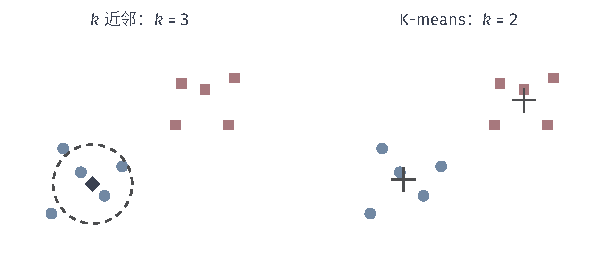
\includegraphics[width=101.406mm]{figures/02-foundations/01-basics/tikz/models-neighbors-prototypes/figure.pdf}
  \caption{两个$k$控制不同的对象。左侧kNN保存十个带标签样本，菱形表示新输入，
  虚线圈内的三个近邻参加投票；右侧K-means用两个中心表示群组。
  固定近邻数不会固定实例总数，固定簇数则固定了中心数量。图为表示方式的教学示意。}
  \label{fig:models-neighbors-prototypes}
\end{figure}

实例预测仍有自己的假设。距离与特征尺度决定邻居身份，$k$决定参考范围；改变尺度可能改变结果，增加实例也增加存储和查询成本。这里保存数据是预测规则的组成。线性回归程序也可能为重新训练或来源追踪保留全部数据，但预测函数仍只需固定权重。因此，应看预测关系必须依赖什么，而不能仅数程序保存了多少文件。

数据增加也可以通过条件规则进入表示。\term{决策树}（decision tree）逐层比较特征阈值，把输入分到区域，再输出区域内的预测。若叶数不设固定上限，更多数据可以支持更多分支，阈值和叶输出的数量也能增长，属于非参数化设定。若固定深度或叶数上限，表示规模就受到固定限制。第\ref{sec:models-nonlinear}节会用平面划分说明这些规则的作用。

\term{随机森林}（random forest）把多棵树的预测合在一起。仅固定树的棵数，还不足以限定总表示规模；只要各树叶数可以增长，仍可采用非参数化设定。棵数与叶数上限同时固定时，规模才受到相应上限约束。因此，一个配置固定，不等于所有自由度都固定。

局部关系还可以通过加权平均表示。\term{核回归}（kernel regression）按输入的距离或相似性加权训练目标；控制邻近范围的带宽是超参数，样本位置和目标却随数据补充。即使带宽不变，新增附近成交记录也可能改变房价预测。这种依赖实例的局部平滑属于非参数化方法；近邻、树与平滑的关系可参见统计学习教材\scite{hastie2009}。

\subsection{半参数化模型}
\label{sec:models-semiparametric}

房价预测可以对不同输入采用不同限制。假设面积作用采用线性系数，而楼龄关系不预定曲线形式；我们希望保留前一项的固定表示，同时让后一项随数据灵活估计。
\term{半参数化模型}（semiparametric model）就把固定有限维的参数化部分与非参数化
部分结合起来。记面积为$x$、楼龄为$z$，一个教学设定是
\begin{equation}
  f_{\beta,g}(x,z)=\beta x+g(z).
  \label{eq:models-semiparametric}
\end{equation}
系数$\beta$描述面积的固定线性作用，未知函数$g$描述楼龄与房价之间的关系，
后者可以用局部平滑等非参数化方法估计。学习时既要确定$\beta$，也要估计整条函数$g$。
命名依据是固定有限维与非参数部分同时存在；参数个数居于两种方法之间，或只有一半参数已知，都不是这里的判断标准。

方法名称也没有唯一决定表示规模。\term{支持向量机}（support vector machine, SVM）依据得分分类，并在训练时要求样本位于边界的适当一侧、保留一定间隔。间隔的几何意义留到第\ref{sec:models-spatial-objectives}节；这里先比较它采用哪一种表示。

固定$d$维输入的线性SVM使用$s(\bm{x})=\bm{w}^{\top}\bm{x}+b$，
预测只需$d$个权重和一个偏置，是固定维数的表示。使用核函数后，还可以用训练样本的贡献写出得分，供我们检查规模如何变化：
\begin{equation}
  s(\bm{x})=\sum_{i\in I_{\mathrm{SV}}}
    a_i\,\kappa(\bm{x}_i,\bm{x})+b.
  \label{eq:models-support-vector-expansion}
\end{equation}
其中$\kappa$是用于计算两个输入之间关系的核函数，$a_i$为学习得到的系数，
$I_{\mathrm{SV}}\subseteq\{1,\ldots,n\}$包含非零系数对应的训练样本索引，
这些样本称为\term{支持向量}（support vectors）。核函数与特征变换的关系见
第\ref{sec:models-nonlinear}节。

高斯核SVM通常没有等价的固定有限维特征表示，支持向量数又可以随样本增加，因此通常采用非参数化判断。某次模型仅保留部分训练样本，可以降低表示规模，却不把整个模型族改为半参数化。固定带宽等超参数也不固定支持向量数。固定次数的多项式核则对应有限维特征，可以用固定权重表示，需要按具体核重新判断。

半参数化SVM要在预测关系中确实保留两种部分，例如用固定系数表示线性趋势，再用非参数化核模型学习修正项，并联合估计两者\scite{smola1998semiparametric}。这样，固定系数与可扩展修正各有职责。线性、一般核与组合形式的容量不能只凭SVM名称推断：应检查特征空间和候选表示。有限的超参数或某次有限的支持向量集合，都不足以代替这项检查。

\section{变量的概率语义}
\label{sec:models-probability}

固定表示规模后，我们仍不知道模型怎样描述结果的不确定性。以明日温度为例，模型可以直接预测$22\,^{\circ}\mathrm{C}$，也可以描述给定气象观测后温度落在各范围的概率，例如集中在$20$至$24\,^{\circ}\mathrm{C}$附近。这里比较的是内部是否建立分布，而非最终只交付点值还是完整分布；分布模型也可以只返回均值。这个区别同样适用于分类、分组与压缩。

\subsection{非概率模型}
\label{sec:models-nonprobabilistic}

先考虑直接给温度值的设定。模型用函数、规则或几何关系取得结果，不为当前变量明确建立分布，这称为\term{非概率模型}（non-probabilistic model）。
在温度预测中，记气象特征为$\bm{x}$、模型参数为$\bm{\theta}$，模型计算
\begin{equation}
  \hat{y}=f_{\bm{\theta}}(\bm{x}).
  \label{eq:models-point-prediction}
\end{equation}
训练时，根据预测温度与实际温度的偏差调整参数；使用时，将新的观测代入函数，得到一个
预测值。例如，输出$22\,^{\circ}\mathrm{C}$表示模型给出的温度预测。这个点值仍没有给出偏离程度的概率，更高或更低温度的可能性需要另外说明。

K-means与PCA也能从几何要求直接建立。前者找中心并让样本靠近所属中心，预测时返回最近中心编号；后者找投影方向，利用少量坐标保留主要变化。中心距离和投影已经规定了计算，不需要先给样本假定概率分布。

因此，温度偏差、簇内距离或重构误差可以直接服务于点预测、分组或压缩。若问题扩展为“温度偏离预测超过两度的概率是多少”，上述输出尚未给出答案，需要额外建立概率关系。

\subsection{概率模型}
\label{sec:models-probabilistic}

相同观测条件下，明日温度仍可能变化。若要描述这些可能结果，我们把温度视为随机变量，给各范围赋概率。\term{概率模型}（probabilistic model）就是
为任务涉及的随机变量及其关系建立概率分布的模型。对于温度预测，可以让函数给出分布的
均值，并用方差描述围绕均值的变化：
\begin{equation}
  y\mid\bm{x}\sim\mathcal{N}\bigl(\mu_{\bm{\theta}}(\bm{x}),\sigma^2\bigr).
  \label{eq:models-linear-gaussian}
\end{equation}
这里$y\mid\bm{x}$表示给定气象特征$\bm{x}$后的温度，$\mu_{\bm{\theta}}(\bm{x})$给出
该条件下的均值；$\bm{\theta}$是均值函数的参数，$\sigma^2>0$是另一个需要从数据中估计的
模型参数，完整参数由二者组成。$\mathcal{N}(\mu,\sigma^2)$表示均值为$\mu$、方差为
$\sigma^2$的高斯分布。
在均值$22\,^{\circ}\mathrm{C}$、标准差$2\,^{\circ}\mathrm{C}$的教学设定中，均值给出中心预测，整个分布还描述偏离它的温度。图\ref{fig:models-point-distribution}对照了这两种预测形式。

\begin{figure*}[htbp]
  \centering
  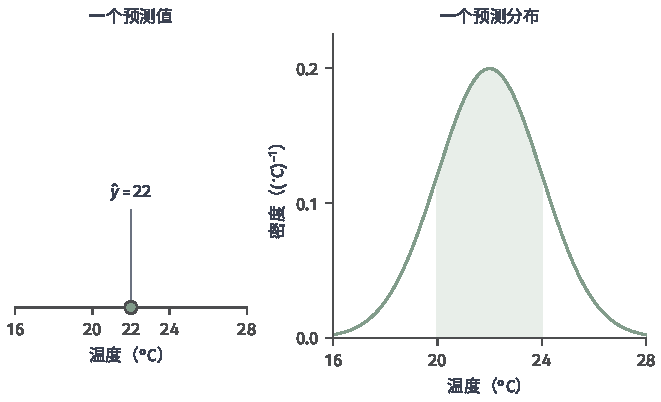
\includegraphics[width=112.000mm]{figures/02-foundations/01-basics/matplotlib/models-point-distribution/figure.pdf}
  \caption{同一温度预测的两种描述。左侧只给出一个预测值；右侧给出高斯预测分布，
  阴影面积表示温度落在$20$到$24\,^{\circ}\mathrm{C}$之间的概率。数值用于教学示意。}
  \label{fig:models-point-distribution}
\end{figure*}

固定聚类问题也可以作同样比较。K-means保存中心并比较距离；\term{高斯混合模型}（Gaussian mixture model, GMM）用多个高斯分布描述样本，每组还有分散程度和总体比例。处于两组之间的样本，前者按最近中心取得组号，后者可以计算各组归属的后验概率。组的大小、形状与重叠因此都参与判断，不只比较中心位置。

降维中的PCA与\term{概率主成分分析}（probabilistic PCA, PPCA）也共享低维目标，却采用不同描述。PCA通过线性投影压缩与重构；PPCA在低维线性表示上加入高斯分布和观测噪声，说明观测怎样分布在子空间附近。在这些假设下，还能估计缺失观测的分布。它增加了观测可能性的描述，而不只是给出投影坐标\scite{tipping1999}。

\paragraph{分类问题的概率建模选择}

给定邮件特征后，类别概率由$p(y\mid\bm{x})$描述。我们已经用逻辑函数直接建立过这种关系；还可以先描述正常与垃圾邮件各自出现哪些特征，再由特征推测类别。两种路线最终回答相同的分类问题，建立的分布对象却不同，分别称为判别式与生成式建模。

\term{判别式建模}（discriminative modeling）直接学习输入与类别之间的关系。概率分类时，候选模型描述$p(y\mid\bm{x})$，逻辑回归便用带标签样本调整权重，使类别概率与观测标签吻合。模型无须同时描述输入特征的总体分布，或每一类内部的特征分布。更广义的判别式路线还包括只学习得分或决策的SVM；这里固定概率输出，以便与另一条路线比较。

另一条路线先规定每类有多常见，以及每类内部输入如何分布。用于分类的\term{生成式建模}（generative modeling）由此建立联合分布
$p(\bm{x},y)=p(y)p(\bm{x}\mid y)$。其中$p(y)$描述各类别的比例，
$p(\bm{x}\mid y)$描述每一类内部的特征分布。训练得到这些分布后，再根据新输入的特征
反推其类别。对于编号为$1,\ldots,k$的类别，由贝叶斯公式得到
\begin{equation}
  p(y=c\mid\bm{x})
  =\frac{p(y=c)\,p(\bm{x}\mid y=c)}
         {\sum_{j=1}^{k}p(y=j)\,p(\bm{x}\mid y=j)}.
  \label{eq:models-generative-classification}
\end{equation}
公式先用$c$类的比例和输入可能性计算其贡献，再除以所有$k$类的贡献之和。分母必须大于零，归一化所得称为类别后验概率。若只需输出概率最大的类别，
比较各类分子即可，因为分母相同。

例如，构造两类邮件比例$p(y=1)=0.2$、$p(y=0)=0.8$，标签$1$仍表示垃圾邮件。假设某组计数$\bm{x}$在两类内部的概率分别为$0.12$与$0.01$。类别比例乘以类内概率，得到联合概率$0.024$与$0.008$，归一化后垃圾邮件概率为$0.024/(0.024+0.008)=0.75$。这个教学计算同时利用了输入对类别的区分和总体类别比例。

\term{朴素贝叶斯}（naive Bayes）按生成式路线估计类内特征分布，增加条件独立假设：给定类别后，一个特征的值不再改变其他特征的分布。该类别内部的特征联合概率便可由各特征的条件概率相乘计算。\term{高斯判别分析}（Gaussian discriminant analysis）也从类内分布出发，但采用多元高斯，能在该模型中保留特征相关性。“生成式”描述的是分布假设的方向：先按$p(y)$取得类别，再按$p(\bm{x}\mid y)$取得特征。在邮件案例中，这些特征只是计数，能够生成计数并不等于能够生成完整正文；后者需要文本分布。

图\ref{fig:models-discriminative-generative}把相同的类别后验放到两条计算路线中。判别式直接学习后验，生成式先学习联合分布再计算后验。下方连续曲线进一步显示，条件类别概率随输入变化，而联合密度同时包含特征分布与类别比例；二者的数值所代表的对象不同。

\begin{figure*}[!htb]
  \centering
  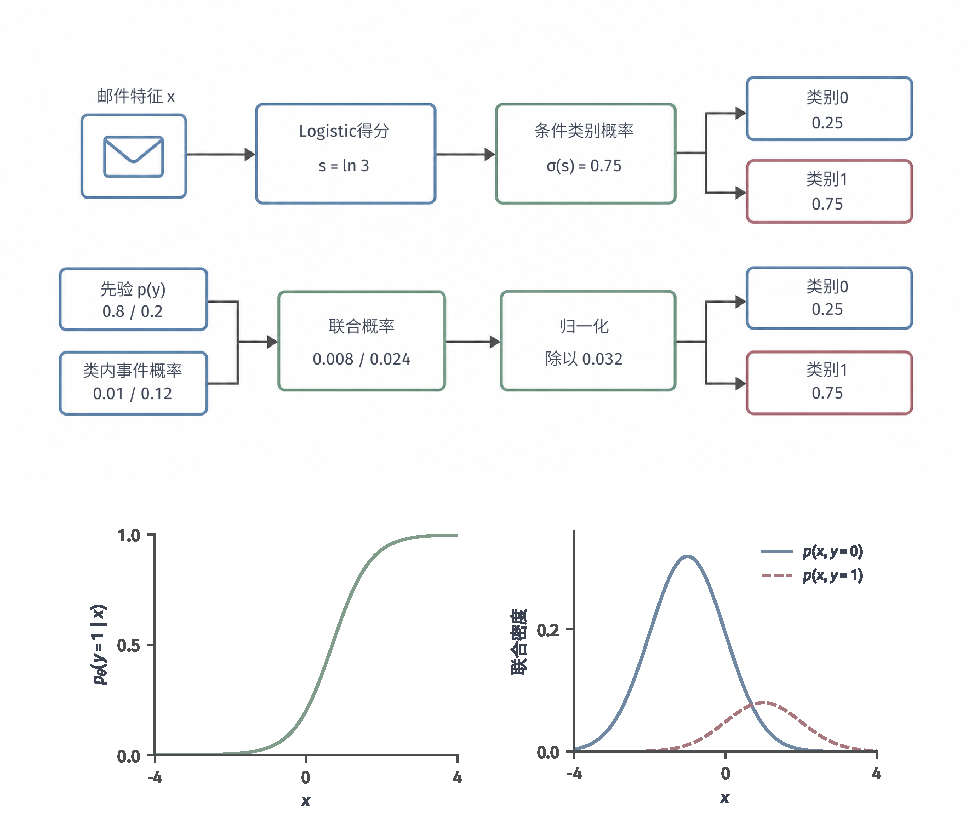
\includegraphics[width=164.600mm]{figures/02-foundations/01-basics/generated/models-discriminative-generative/figure.pdf}
  \caption{两条分类建模路线。上部框图中的判别式路线以二分类Logistic读出为例，令得分$s=\ln3$，则$\sigma(s)=0.75$，得到类别后验$p(y=1\mid x)=0.75$、$p(y=0\mid x)=0.25$。生成式路线沿用离散邮件教学数值，先验$0.8$、$0.2$与类内事件概率$0.01$、$0.12$相乘，分别得到联合概率$0.008$、$0.024$，再除以总和$0.032$。两条路线的数值仅作可核算示意，不假定实际训练结果相同。下方两个面板另用连续构造：先验$0.8$、$0.2$分别对应$\mathcal N(-1,1)$、$\mathcal N(1,1)$。左面板为条件类别概率，右面板为先验加权的联合密度，整个实数轴上的两条密度曲线面积分别为$0.8$与$0.2$；这些密度值不与上部离散事件概率对应。}
  \label{fig:models-discriminative-generative}
\end{figure*}

训练时也要按所建立的对象评价概率。对独立同分布的带标签样本，判别式负对数似然使用$p_{\bm\theta}(y_i\mid\bm x_i)$，生成式则使用$p_{\bm\theta}(\bm x_i,y_i)$。即使最后的类别后验具有相同形式，拟合不同概率对象仍可能产生不同参数。前者集中估计类别关系；后者描述范围更广，在假设成立时还能采样或补全，同时也要估计更多关系\scite{ng2001}。

得到类别或区间概率还需要处理参数是否已知。第一卷“随机变量”章已建立\term{概率推断}（probabilistic inference）、\term{似然}（likelihood）、\term{最大似然估计}（maximum likelihood estimation）和贝叶斯后验；这里把这些工具放回模型使用过程。参数给定时，
可以从模型分布计算类别概率、区间概率等所需结果。参数未知时，一种做法是用
\term{点估计}（point estimation）从观测到的训练数据$\mathcal D$选出
$\hat{\bm{\theta}}$，再使用插件预测$p(y\mid\bm x,\hat{\bm{\theta}})$；另一种做法是用
\term{贝叶斯推断}（Bayesian inference）从\term{先验分布}（prior distribution）得到
\term{后验分布}（posterior distribution），并对不同参数对应的预测分布加权平均。
记$\Theta$为参数的允许范围。在新结果$y$给定$\bm x$和$\bm\theta$后与$\mathcal D$
条件独立的常见设定下，后验预测写为
\[
  p(y\mid\bm x,\mathcal D)
  =\int_{\Theta} p(y\mid\bm x,\bm\theta)
    p(\bm\theta\mid\mathcal D)\,\mathrm d\bm\theta.
\]
插件预测固定一个估计参数，后验预测则对允许参数集合中的预测按后验权重求平均。求和或积分的对象是参数不确定性；使用者最终取得点值、摘要或完整分布，还由输出接口决定。
即使参数完全给定，模型中的随机结果仍可变化；传播参数后验也不能免除区间覆盖的实际检验。如何检验这些概率输出
由第~\ref{chap:trust-reliability}章负责；复杂依赖下的推断算法则由
\BookPartRef{part:probabilistic-models}{第三卷“模型”的“概率图模型”部分}
作为\term{概率图模型}（probabilistic graphical model）专题展开。

上述参数处理方式并没有决定表示规模。成分数固定的GMM可以用固定维数参数描述，是参数化概率模型；高斯过程描述一组可能函数上的概率关系，通常属于非参数化概率模型\scite{rasmussen2006}。两个维度仍需分别判断。

\paragraph{概率描述带来了什么}

概率信息的用途可以从同一个温度预测看出。两个模型都给出中心值$22\,^{\circ}\mathrm{C}$，一个集中在$21$至$23\,^{\circ}\mathrm{C}$，另一个允许更宽的变化。对温度敏感的活动，这两项分布支持不同的风险判断。聚类也一样：GMM若给某样本近乎相同的两个组别后验，仅取较大者可以作出选择，却没有消除归属的不确定性。

取得分布之后，还需要检验它与未参与训练的结果是否相符。模型给出名义覆盖概率$90\%$的区间时，可以统计实际温度进入区间的比例。在同一组独立评价数据上，两个区间的实际覆盖率相近时，较窄的区间一般提供更具体的信息；无限放宽区间虽容易包含真实温度，却未必支持决策。因此，应同时检查预测位置和不确定性范围，不能只看中心误差或只看覆盖。

检验也可能暴露分布形状的限制。例如，同类条件下温度出现两个峰时，单个高斯的均值可能位于二者之间，区间并不能合适地反映观测规律。错误的群组形状也会影响聚类后验。引入概率只增加了描述不确定性的方式，任务是否获得收益，仍要由假设与数据是否吻合、分布估计是否可靠来决定。

\section{变量的关系形式}
\label{sec:models-structure}

相同输入和输出类型，仍然可以采用不同的计算关系。温度可能随某个特征按固定幅度变化，也可能在不同范围按不同规律变化。模型结构描述的就是这项选择。回归可检查预测函数，分类可检查得分或边界，降维可检查坐标映射；判断线性以前，必须先固定正在考察哪一个量。

\subsection{线性结构}
\label{sec:models-linear}

先固定其他特征，假设一个特征每增加一单位都带来相同预测增量。线性回归用权重记录这种增量，将$d$维输入$\bm{x}$与$\bm{w}\in\mathbb{R}^{d}$加权相加，再加偏置$b$：
\begin{equation}
  \hat{y}=\bm{w}^{\top}\bm{x}+b
  =\sum_{j=1}^{d}w_jx_j+b.
  \label{eq:models-linear-score}
\end{equation}
固定其他特征后，$x_j$每增加一个单位，预测值都改变$w_j$。
例如，用面积预测房价时，线性关系假设每增加一平方米带来的预测增量相同。
严格说，带常数项$b$的关系称为仿射关系；机器学习中通常也将它归入线性模型。

分类概率不能直接使用任意实数得分。逻辑回归通过转换函数把得分放到零与一之间。记二分类正类概率为$p$，计算及其等价变形为
\begin{equation}
  p=\frac{1}{1+\exp[-(\bm{w}^{\top}\bm{x}+b)]},
  \qquad
  \log\frac{p}{1-p}=\bm{w}^{\top}\bm{x}+b.
  \label{eq:models-logistic-structure}
\end{equation}
左式将任意实数得分转为零与一之间的概率。右式来自对左式的变形：$p/(1-p)$比较正类
与负类的概率大小，再取对数，就得到\term{对数几率}（log odds）。这个量仍然是输入
的仿射函数。用$p=0.5$作分类阈值时，两类概率相等，对数几率为零，边界因而满足
$\bm{w}^{\top}\bm{x}+b=0$，在二维平面中就是一条直线。
所以这里把逻辑回归称为线性分类模型时，指的是对数几率或分界关系，概率本身仍经过非线性转换。

逻辑回归的线性指对数几率和分类边界，线性回归的线性则指预测值。基础\term{感知机}（perceptron）也计算加权得分，再按正负分类。感知机与线性SVM学习参数的准则不同，却都用线性分界面完成二分类，因此关系形式不能替代训练准则的比较。

PCA也使用线性关系，只是对象改为投影坐标。均值与方向固定后，每个坐标都是中心化输入的加权和。PPCA加入分布与噪声假设，仍保留低维表示到观测均值的线性关系。因此，这项结构选择可以用于预测、分类、降维和概率建模，并不专属某一个任务。

K-means没有预先给类别边界，但最近中心规则会产生分配区域。为找出两个区域之间的分界，取中心
$\bm{\mu}_1$与$\bm{\mu}_2$，边界上的样本满足
$\lVert\bm{x}-\bm{\mu}_1\rVert_2^2=\lVert\bm{x}-\bm{\mu}_2\rVert_2^2$。
展开两边并消去共同的$\bm{x}^{\top}\bm{x}$项，得到
\begin{equation}
  2(\bm{\mu}_2-\bm{\mu}_1)^{\top}\bm{x}
  =\lVert\bm{\mu}_2\rVert_2^2-\lVert\bm{\mu}_1\rVert_2^2.
  \label{eq:models-kmeans-boundary}
\end{equation}
消去平方项后得到输入的仿射方程，说明两个不同中心之间的分配边界是线性的。距离本身仍是二次函数，输出的离散编号也不能解释为输入的线性函数。
后文将K-means放在线性一侧时，专指这种两两分配边界。

输入表示改变后，线性判断也可能改变。先把$x$变成$x^2$，再计算$wx^2+b$，对新特征是线性的，对原始$x$却不是。本章主要以原始输入为基准。参数的线性出现方式也属于另一个观察对象，不能与预测对输入的线性混为一谈。

\subsection{非线性结构}
\label{sec:models-nonlinear}

固定增量假设未必适合当前对象。速度增加时，刹车距离通常不按同一增量改变；剂量作用可能随区间改变；促销词的含义还可能依赖外部链接数。我们要表达的于是包括弯曲、阈值和特征共同作用，单个仿射关系未必充分。

保持上一节的观察对象，如果预测值或得分不能写成原始输入的仿射函数，就称这一关系为非线性。二分类若需要弯曲或分段边界，也不能只用一个超平面。图\ref{fig:models-linear-nonlinear}固定同一组中心与外圈样本作比较：任何直线都无法完全分开两类，径向边界却可以。差别来自候选关系，而不是更换了评价样本。

\begin{figure*}[!ht]
  \centering
  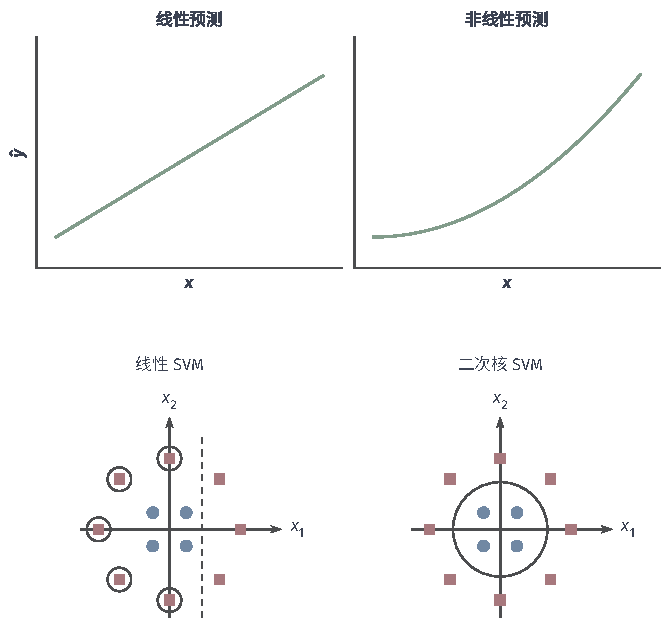
\includegraphics[width=112.000mm]{figures/02-foundations/01-basics/tikz/models-linear-nonlinear/figure.pdf}
  \caption{线性与非线性关系的几何示意。上排依次为线性预测与非线性预测，
  下排用同一组环形样本对照线性SVM的限制与二次核SVM的表达能力；圆点和方点代表两类。
  左图虚线只展示一条候选直线，空心圈标出按其左右类别分配时的错分方点，不代表最优SVM解。
  外圈方点的凸包包含内圈圆点，故任何直线都不能完全分离这组样本。
  右图以圆心为坐标原点，半径$8$的边界可由二次核
  $\kappa(\bm u,\bm v)=(\bm u^{\top}\bm v)^2$与偏置表示。图为几何构造，非训练结果。}
  \label{fig:models-linear-nonlinear}
\end{figure*}

曲线能弯曲，并没有同时规定其他维度。固定次数的多项式回归只需固定系数，是参数化的非线性模型；高斯过程同样能产生弯曲关系，却对函数建立概率分布，并不受固定有限维系数限制。因此，图形只显示关系形式，表示规模和概率语义仍需另外考察。

多个特征也可以共同决定变化。关系中出现$x_1x_2$时，改变$x_1$的作用会随$x_2$而变，称为特征交互。例如，可以规定只有邮件带有外部链接时，新增促销词才提高怀疑得分；不带链接时，促销词的权重为零。两个计数的固定权重和无法令同一项的权重随另一项改变。分别观察每个特征可能看不到这一点，需要把它们放到共同关系中比较。

是否扩大表示，需要任务数据提供依据。线性关系给出了固定特征增量的基线；若独立验证样本显示，模型在某些输入范围持续高估、在另一些范围持续低估，或误判集中于特定特征组合，就需要检查固定增量假设是否遗漏了弯曲、阈值或交互关系。增加分段规则或非线性变换，是针对这些具体偏差扩展候选表示，效果仍需验证。表达范围扩大，也更容易迎合偶然波动，需要配合数据量和结构限制判断。下面比较按条件划区与改变特征这两种实现方式。
\FloatBarrier

\paragraph{按条件采用不同规则}

我们可以先确定输入落在哪个区域，再按区域使用规则。决策树把这一步写成连续条件判断，例如促销词达到阈值后再检查链接数。根到叶的路径汇集了输入要满足的条件，叶节点给出对应区域的预测。图\ref{fig:models-tree-partition}把相同条件同时画成判断树和平面区域，以便直接对照。

\begin{figure}[htbp]
  \centering
  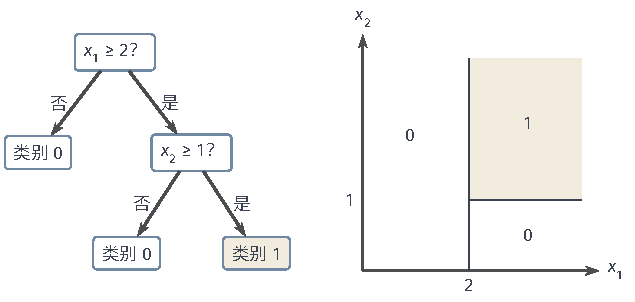
\includegraphics[width=\linewidth]{figures/02-foundations/01-basics/tikz/models-tree-partition/figure.pdf}
  \caption{按条件分情况处理输入。左侧为判断树，右侧为对应的输入区域。
  该教学例子在$x_1\geq2$且$x_2\geq1$时输出类别$1$，其余区域输出$0$。}
  \label{fig:models-tree-partition}
\end{figure}

单个特征阈值只划分两侧，多次组合却能形成复杂区域。常见树在叶节点给固定输出，跨过区域边界时预测可能跳变。这种结构适合表达条件规则，但表示规模还取决于叶数：允许随数据增长是非参数化设定，固定上限则限制候选规模。非线性的分支结构与参数化方式因此需要分开判断。

\paragraph{对输入进行非线性变换}

另一种方式先保留能表达变化的特征，再计算得分。平方项$x_1^2$可以表示弯曲，乘积$x_1x_2$可以表示交互。把变换记为$\bm{\phi}(\bm{x})$，在新特征上使用线性得分：
\begin{equation}
  s(\bm{x})=\bm{w}^{\top}\bm{\phi}(\bm{x})+b.
  \label{eq:models-feature-score}
\end{equation}
变换中的非线性关系可能使这个线性得分在原空间形成非线性边界。
例如，中心区域是一类、外围是一类时，可以把到原点的平方距离
$x_1^2+x_2^2$作为新特征，再用一个阈值区分两类。

\term{核方法}（kernel methods）借助特征空间内积使用变换后的关系，无须逐一写出所有特征。线性核仍对应线性关系，高斯等非线性核可以形成弯曲边界。标准高斯核SVM可以随样本保留更多系数，采用非参数化表示；若先固定有限个变换特征作近似，就改变了候选规模的设定\scite{cortes1995}。

手工加入平方项和交互项，仍需要预先选择变换。神经网络让中间变换也由训练确定：多层网络在加权和之间加入\term{激活函数}（activation function），例如把负值置零、保留非负值，使不同输入范围有不同计算关系。训练目标共同调整这些中间表示和最终预测。如果各层都只有加权和与偏置，把一层代入下一层仍得到仿射函数；单纯堆叠这样的层，并不会扩大到非线性关系。

树按条件改变规则，特征变换则让新的坐标表达弯曲与交互。两种思路可以交叉，分段线性网络也能形成不同计算区域。无论采用哪一种，结构只说明可表达什么，新样本上的效果还要由数据、限制与训练方式支持。

计算图和概率图都用节点与边组织变量，但读图时要依据各自的语义。神经网络中的边规定一个数值怎样进入后续计算；概率图中的边参与规定局部概率分解，而条件独立关系要按照该类图的判定规则读取。边的存在允许直接联系，缺边所表达的独立性则依赖图的语义及模型假设。这两种组织方式可以结合：用神经网络计算某个分布的参数，既保留非线性计算，又建立概率描述。

\FloatBarrier
\section{输出的形式与含义}
\label{sec:models-output}

设定了模型内部的计算关系以后，我们还要决定把哪些结果交给使用者。温度预测可以只返回一个数，也可以提供预测区间或完整分布；邮件分类可以直接返回类别，也可以同时列出类别概率。因此，说明输出需要分两步：先说明结果按标量、向量还是位置与顺序构成的对象组织，再说明其中数值代表预测值、类别编码、分布摘要、完整分布还是采样结果。只给出形状，使用者仍不知道这些数怎样用于判断。

\subsection{输出的组织形式}
\label{sec:models-output-form}

\paragraph{标量输出}
\label{sec:models-scalar-output}

温度预测若只返回$22\,^{\circ}\mathrm{C}$，结果便由一个数及其单位构成。价格预测和商品评分也常采用这种\term{标量输出}（scalar output）。使用时，数值必须连同单位或评分尺度一起解释。

一个数也可以用作编号。邮件分类中的$0$与$1$可分别表示正常邮件和垃圾邮件，聚类中的$1,2,\ldots,k$则区分发现的群组。前者的含义由预先定义的标签确定，后者的含义来自分组结果。交换簇编号不会改变哪些样本同属一组，因而编号之差通常不能解释为距离。

\paragraph{向量与结构化输出}
\label{sec:models-vector-output}

同时预测温度、湿度和风速时，单个数已经容纳不了全部结果，我们需要按约定次序返回三个分量。这便是\term{向量输出}（vector output）。未来七天的温度也可以组成向量，不过此时分量依次对应日期。使用任何这样的结果，都要知道各坐标对应的对象、单位和顺序。

向量还可以描述输入，而不直接给出任务答案。PCA的输出坐标记录样本沿各投影方向的位置，神经网络也可以把图像映射成用于检索或分类的特征向量。同一图像经过裁剪、颜色变换等处理得到的输入版本称为\term{视图}（view）。若这些变换按任务设定保留内容含义，训练便可以要求不同视图的表示在指定距离或相似度下接近；这里需要保留的是表示之间的关系。

重构图像时，输出虽也是一组数值，却必须按像素位置和颜色通道还原成数组。文本则要保留符号顺序，还可能具有不同长度。对于这些结构化结果，分量值与位置、顺序或连接关系共同决定含义，不能任意交换坐标。

组织形式确定以后，输出含义仍需单独说明。三个数可以是三个温度预测，也可以是三个类别的概率；后一种解释额外要求分量非负且总和为一。一个数也可能是测量值或类别编号。下面我们据此区分直接结果、分布摘要和概率分布，说明同样形状的接口可以提供哪些不同信息。

\subsection{输出的含义}
\label{sec:models-output-semantics}

第\ref{sec:models-probability}节判断模型是否为变量建立分布。这里转而查看使用者实际收到什么：模型可能交付完整分布，也可能只返回由它计算的类别、均值或区间。模型内部保留的信息与接口交付的信息应分别说明。

\paragraph{点结果与分布摘要}

直接结果可以是一个预测值、类别或簇编号。即使内部建立了概率分布，接口也可以只返回摘要：逻辑回归选出概率最大的类别，高斯温度模型报告均值或预测区间。摘要使比较与决策更方便，却省略了部分可能结果及其概率。因此，输出一个点或区间，并不能据此判断模型内部有无概率语义。

\paragraph{概率分布与采样}
\label{sec:models-distribution-output}

若使用者需要比较各个结果的可能性，接口就应保留\term{概率分布输出}（probability distribution output）。有限类别可以逐项列出非负且总和为一的概率。例如，邮件分类的$(0.2,0.8)^{\top}$分别给正常邮件和垃圾邮件赋予$0.2$与$0.8$。它比单个类别标签多保留了概率如何分配的信息。不过，这些数能否对应实际频率，还要通过校准检验，不能仅凭概率集中就宣称预测可靠。

连续结果通常无法逐个列出概率，而是通过分布形式及其参数说明。例如，指定高斯分布并给出均值$22$、方差$4$，就确定了温度的密度曲线。某一区间对应的曲线下面积才是落入该区间的概率；单点的曲线高度是密度，不能当作恰好取该值的概率。

一个概率模型由此可以提供三种接口：交付分布、计算摘要，或从分布采样。温度模型可以报告均值$22\,^{\circ}\mathrm{C}$，也可以给出包含指定模型概率质量的预测区间；后者的名义概率水平是否达到实际频率覆盖，需要另用未参与训练的数据检查。一次采样则可能返回$21.3\,^{\circ}\mathrm{C}$。图像生成也遵循这个区别：分布描述可能图像，采样才产生一张具体图像，多次采样可以产生不同结果。

因此，输出形状与输出含义要配合解释。类别分布可以写成向量，分布均值可以是标量，采样结果可以是高维数组。明确返回几个分量以后，我们还要交代它们是直接答案、分布的概括、完整概率描述，还是一次实现结果。

\section{损失与学习准则}
\label{sec:models-objectives}

模型能够表示和输出一个结果，接下来需要说明它怎样借助数据作出选择。邮件分类和聚类都可返回编号，但分类已有正确标签，可以比较预测与答案；聚类没有逐样本标签，需要从样本之间的关系规定分组依据。对于要拟合的模型，我们必须给出评价候选结果的准则；对于没有显式参数拟合目标的方法，则要说明实际形成输出的规则。

本节从评价所用的信息展开。逐样本答案已知时，我们比较数值、向量或概率分布与目标的差异；答案缺失或任务还关心对象之间的关系时，我们规定紧凑性、分类间隔、相对邻近或低维结构；行动会改变后续结果时，评价需要延伸到轨迹和长期收益。这些准则可以组合，例如PCA在低维限制下减小重构误差。没有显式拟合目标的方法应标明这一情况，不能把保存或查询步骤写成损失。

\subsection{逐样本的目标差异}
\label{sec:models-pointwise-objectives}

先看每个样本都有答案的任务。温度、价格与销量预测有待预测的真实数值，分类有真实类别，但两类答案所需的比较方式不同。记第$i$个样本的答案为$y_i$、预测为$\hat y_i$，我们通常先计算单个样本的损失，再在$n$个样本上求平均，以评价模型整体表现。

\paragraph{连续数值}

预测高于真实温度两度与低于真实温度两度，都偏离两个单位。直接累加带符号误差会使二者抵消，我们可以改用平方或绝对值计算损失：
\[
  \ell_{\mathrm{sq}}(\hat y,y)=(\hat y-y)^2,\qquad
  \ell_{\mathrm{abs}}(\hat y,y)=|\hat y-y|.
\]
在样本上求平均，分别得到第~\ref{sec:performance-measures}节的均方误差与平均绝对误差。真实值为$20$、预测为$22$时，单个平方误差为$4$，绝对误差为$2$；偏差从$2$增至$4$时，二者分别增至四倍和两倍。因此，平方误差更强调大偏差，作为预测值的函数也处处可导；绝对误差对个别大偏差的影响较小，但在零误差处不可导，优化需作相应处理。

误差的两个方向还可能具有不同代价。备货不足会造成缺货，备货过多会增加库存成本，二者未必应受相同惩罚。此时损失要分别反映高估和低估的后果，而不只是笼统要求数值接近。

\paragraph{离散类别}

类别编号表示身份，而非连续尺度。若$1$、$2$、$3$分别代表猫、狗、鸟，编号之差无法评价误判严重程度。\term{零一损失}（zero-one loss）因此只检查预测与真实类别是否相同：
\begin{equation}
  \ell_{01}(\hat{y},y)=
  \begin{cases}
    0, & \hat{y}=y,\\
    1, & \hat{y}\ne y.
  \end{cases}
  \label{eq:models-zero-one-loss}
\end{equation}
其样本平均即分类错误率。但只要预测类别不变，参数怎样微调都不会改变这个损失，它难以指引连续参数更新。训练时常采用随得分或概率变化的\term{代理损失}（surrogate loss），如后文的类别交叉熵和第\ref{sec:models-spatial-objectives}节的间隔损失，以便优化。若误判类型的代价不同，还可以用预先给定的代价表替代统一的$1$。

\paragraph{向量的差异}
\label{sec:models-vector-objectives}

图像去噪要比较输出图像与干净图像，重构要比较恢复结果与原输入，多变量预测则要同时比较多个观测量；它们的答案都是向量。表示学习也比较向量，例如让同一图像的不同视图在指定度量下接近。前一类任务常关心每个分量能否恢复，后一类可能主要关心整体方向或相对位置，因此不能只凭向量形式选定损失。

设预测为$\hat{\bm y}$，目标为$\bm y\in\mathbb R^m$。逐分量比较可采用
\begin{align}
  \ell_2(\hat{\bm{y}},\bm{y})
    &=\lVert\hat{\bm{y}}-\bm{y}\rVert_2^2
      =\sum_{j=1}^{m}(\hat{y}_j-y_j)^2,
    \label{eq:models-vector-loss}\\
  \ell_1(\hat{\bm{y}},\bm{y})
    &=\lVert\hat{\bm{y}}-\bm{y}\rVert_1
      =\sum_{j=1}^{m}|\hat{y}_j-y_j|.
    \label{eq:models-vector-l1}
\end{align}
第一式累加平方偏差，大误差获得较高权重；第二式累加绝对偏差，个别异常分量的影响较小。两者都受坐标尺度影响，同时比较温度与气压时，就需要决定是否缩放分量或设置权重。

若关心向量方向而非长度，我们可以比较夹角的\term{余弦相似度}（cosine similarity），方向越接近，相似度越大。对非零向量$\bm a$、$\bm b$，将它转为要最小化的损失可写成
\begin{equation}
  \ell_{\mathrm{cos}}(\bm{a},\bm{b})
  =1-\frac{\bm{a}^{\top}\bm{b}}
          {\lVert\bm{a}\rVert_2\lVert\bm{b}\rVert_2}.
  \label{eq:models-cosine}
\end{equation}
$(1,2)^{\top}$与$(2,4)^{\top}$虽长度不同，但同向，因而余弦损失为零，欧氏误差却非零，见图\ref{fig:models-vector-comparison}。这种忽略长度变化的比较可用于某些文档或图像表示；若幅度本身代表温度、亮度或数量，它也会漏掉任务所需的信息。

\begin{figure}[htbp]
  \centering
  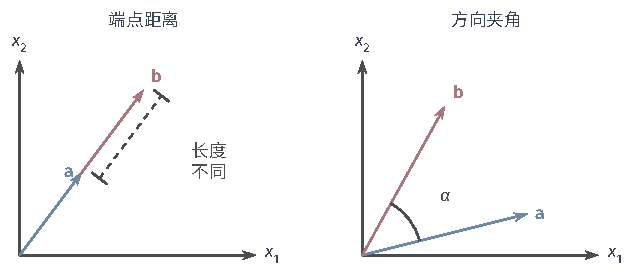
\includegraphics[width=\linewidth]{figures/02-foundations/01-basics/tikz/models-vector-comparison/figure.pdf}
  \caption{两种向量比较方式关注不同差异。左侧比较两个端点之间的距离，
  右侧比较向量方向之间的夹角。同向但长度不同的向量，余弦损失为零，欧氏误差仍大于零。}
  \label{fig:models-vector-comparison}
\end{figure}

数值误差是否符合任务中的相似性，还取决于所用表示。一张图像只平移一个像素，内容可能基本相同，许多对应像素却已有较大差异。位置必须精确对应的重构适合逐像素比较；关心物体内容的任务则可能先提取特征，再比较表示。选择度量时，我们也在选择要保留哪些差别。

\paragraph{概率分布的差异}
\label{sec:models-probability-objectives}

概率输出包含的信息多于最终类别或均值。邮件分类可能还要求概率能够用于风险判断，分布学习要描述样本出现的规律，模型模仿则可能要求两个模型对各类别给出相近概率。面对这些任务，只比较选出的答案会漏掉其余概率信息，我们需要评价分布本身。

有限类别的概率分布可以逐项比较。正式定义及条件见\BookSectionRef{sec:information-log-score-kl}{第一卷“信息论与统计几何”章的“对数评分与KL散度”一节}和\BookSectionRef{sec:statistics-scoring-calibration}{第一卷“随机变量”章的“评分与校准”一节}，这里说明它们怎样接入模型。设目标$\bm p=(p_1,\ldots,p_k)^{\top}$、预测$\bm q=(q_1,\ldots,q_k)^{\top}$均非负且各自求和为一。模型给结果$j$的概率越低，$-\log q_j$越大；以目标概率$p_j$加权平均，便得到\term{交叉熵}（cross-entropy）：
\begin{equation}
  \operatorname{CE}(\bm{p},\bm{q})=-\sum_{j=1}^{k}p_j\log q_j.
  \label{eq:models-cross-entropy}
\end{equation}
已知样本类别为$c$时，可以把目标写成$p_c=1$、其余为零的\term{独热表示}（one-hot representation），损失于是化为$-\log q_c$。给正确类别$0.9$比$0.1$产生的损失小，而$q_c$趋近零时损失趋向无穷大，故自信的错误受到较重惩罚。本节使用自然对数。

预测分布与目标分布相同，交叉熵仍可能为正，因为目标本身可能有不确定性。若要把完全相同的分布记为零差异，就需从交叉熵中扣除目标分布对自身的交叉熵。

扣除目标自身的交叉熵，得到\term{KL散度}（Kullback--Leibler divergence）：
\begin{equation}
  D_{\mathrm{KL}}(\bm{p}\Vert\bm{q})
  =\sum_{j=1}^{k}p_j\log\frac{p_j}{q_j}.
  \label{eq:models-kl}
\end{equation}
其中$p_j=0$的项约定为零，$p_j>0$而$q_j=0$时取无穷大。散度非负，且仅在两个分布相同时为零。把式\eqref{eq:models-kl}中的对数比值拆开，可得$D_{\mathrm{KL}}(\bm p\Vert\bm q)=\operatorname{CE}(\bm p,\bm q)-\operatorname{CE}(\bm p,\bm p)$；目标固定时，后一项不随预测改变，因此两种准则的最小化要求相同。交换目标与预测会改变加权所依据的分布，KL散度一般也会改变。

也可以把预测概率与观测类别的独热向量直接比较。类别为$c$时，$\bm e_c$仅第$c$项为1，\term{Brier评分}（Brier score）写为
\begin{equation}
  \ell_{\mathrm{Brier}}(\bm{q},c)
  =\sum_{j=1}^{k}(q_j-\mathbb I\{j=c\})^2.
  \label{eq:models-brier}
\end{equation}
按这个求和定义，评分在$0$到$2$之间。真实类别分布为$\bm p$时，其期望可分成不依赖$\bm q$的不可约项与$\|\bm q-\bm p\|_2^2$，所以$\bm q=\bm p$取得最小值。它对极端错误的惩罚有上限，交叉熵则没有，两者由此赋予少数自信错误不同权重。Brier评分既可训练也可评价概率预测，是较早提出的概率预报准则之一\scite{brier1950}。

学习数据分布时，我们通常只掌握样本，并不知道真实分布。对模型密度$p_{\bm\theta}(\bm x)$，可以最小化平均负对数似然：
\begin{equation}
  \ell_{\mathrm{NLL}}(\bm{\theta})
  =-\frac{1}{n}\sum_{i=1}^{n}\log p_{\bm{\theta}}(\bm{x}_i).
  \label{eq:models-negative-log-likelihood}
\end{equation}
它鼓励模型对已观测样本给出较大的概率或密度，GMM等分布模型可以使用这一目标。若真实分布$P$和模型$Q_{\bm\theta}$相对共同参考测度有密度，且$P\ll Q_{\bm\theta}$、有关对数期望存在，总体期望负对数似然就是交叉熵；固定$P$后，最小化它等价于在模型类内减小$D_{\mathrm{KL}}(P\|Q_{\bm\theta})$。模型失配时只能得到类内最优近似；有限样本的经验优化还需一致收敛或估计条件，不能只凭独立同分布抽样推出总体最优。若$y$是有限类别标签，拟合$p_{\bm\theta}(y\mid\bm x)$时，相应负对数似然就是分类交叉熵。

目标固定时，交叉熵与KL散度的最小化要求相同；Brier评分则限制了极端错误所受的惩罚。这些准则依据各结果的概率进行比较，并不自动知道两个类别或位置相距多远。若任务关心概率质量移动的距离，还需要把结果空间中的距离纳入准则。

\subsection{关系与结构准则}
\label{sec:models-spatial-objectives}

没有逐样本答案时，我们可以规定对象应当怎样组织；已有答案时，任务也可能在逐样本正确之外提出关系要求。聚类要求同组样本紧凑，检索要求相关样本更近，分类可以要求正确一侧的样本还离边界足够远，降维则限制表示所在空间的维数。这些关系与结构准则比较的对象各不相同；其中有些是必须满足的约束，有些是通过损失鼓励的性质。

\paragraph{样本到中心的距离}

K-means选择$k$个中心，让每个样本与最近中心的平方距离尽量小：
\begin{equation}
  \min_{\bm{\mu}_1,\ldots,\bm{\mu}_k}
  \frac{1}{n}\sum_{i=1}^{n}\min_{1\leq j\leq k}
  \lVert\bm{x}_i-\bm{\mu}_j\rVert_2^2.
  \label{eq:models-kmeans-objective}
\end{equation}
内层在固定中心下为样本选择归属，外层改变中心位置以缩小平均距离。簇编号来自这一几何准则，没有真实类别作参照。平方距离提高远点的影响，偏好围绕中心的紧凑群组。若换成$L_1$距离，固定分组后的最优中心为各坐标中位数，对少数远点通常更稳健；若方向更重要，则可另选基于余弦相似度的准则。

K-means的目标只直接缩小簇内平方距离，并未要求每两个簇都尽量远离。中心取各簇均值时，总平方离差可以分为簇内项与簇间项；固定数据后，前者减小会使后者增大。不过，簇间项衡量各中心相对总体均值的分散程度，不能保证所有簇对都充分分离。

\paragraph{样本到分类边界的间隔}

SVM在预测正确之外还要求留出\term{间隔}（margin）：样本应位于边界正确一侧，并与边界保持余量。令$y\in\{-1,+1\}$，得分$f(\bm x)=\bm w^{\top}\bm x+b$，常用\term{合页损失}（hinge loss）为
\begin{equation}
  \ell_{\mathrm{hinge}}(y,f(\bm{x}))
  =\max\{0,1-yf(\bm{x})\}.
  \label{eq:models-hinge}
\end{equation}
得分满足$yf(\bm x)\ge1$时损失为零，错误分类或余量不足则受到惩罚。不过，单纯放大得分就可能降低该损失，而边界位置未变。线性SVM还惩罚$\|\bm w\|_2^2$：当$\bm w\ne\bm0$时，有符号几何距离为$yf(\bm x)/\|\bm w\|_2$；固定得分余量为$1$，较小权重范数对应较大几何间隔。损失与惩罚共同权衡余量违反及间隔大小，无需把全部同类样本压到一个中心附近。

\paragraph{相关样本之间的相对距离}

检索有时只需要保留相对次序：同一物体的两张照片应比不同物体的照片更近。令参照表示为$\bm a$、相关表示为$\bm p$、不相关表示为$\bm n$，指定距离$d$及余量$m>0$，\term{三元组损失}（triplet loss）比较两段距离：
\begin{equation}
  \ell_{\mathrm{triplet}}
  =\max\{0,d(\bm{a},\bm{p})-d(\bm{a},\bm{n})+m\}.
  \label{eq:models-triplet}
\end{equation}
相关样本至少近$m$时，损失为零，否则不足的差额计入损失。它规定相对关系，不要求表示围绕固定中心。效果依赖距离、样本配对和余量：容易满足的比较少有学习信号，错误配对会促成错误邻近关系。图\ref{fig:models-spatial-objectives}对照中心距离、分类间隔与相对距离；依据已知相似关系学习表示或距离，是\term{度量学习}（metric learning）的基本思路\scite{weinberger2009}。

\begin{figure*}[t]
  \centering
  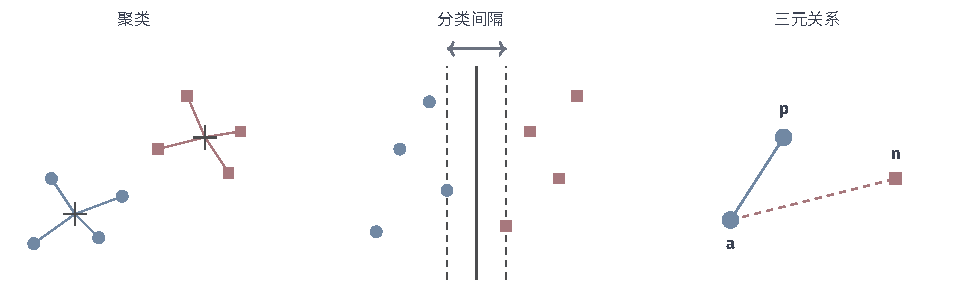
\includegraphics[width=161.406mm]{figures/02-foundations/01-basics/tikz/models-spatial-objectives/figure.pdf}
  \caption{三种几何要求。左侧缩短样本到所属中心的距离；中间让带标签样本与分类边界保持
  间隔；右侧要求相关样本比不相关样本更接近参照样本。三者分别比较不同的几何对象。}
  \label{fig:models-spatial-objectives}
\end{figure*}

PCA提供另一种组织要求：先把表示限制在低维空间，再减小重构误差。将它与上述例子对照，中心距离要保留紧凑群组，分类间隔要保留边界余量，相对距离要保留邻近次序，低维约束要压缩表示。选用哪一种，取决于任务需要保留什么；一个模型也可以同时满足几种要求。

\FloatBarrier
\subsection{轨迹与长期目标}
\label{sec:models-sequence-objectives}

机器人导航中的一步不能只按眼前离终点有多近评价：看似向前的动作可能进入死路，暂时绕行却可能更早到达。游戏决策和连续资源调度也会由当前动作改变后续状态与奖励。我们因而需要评价整段行动，并考虑环境与动作选择可能产生的不同经历。

动作规则与环境共同决定一条轨迹。常见评价先累计轨迹中的多步奖励，再对可能轨迹取期望；另一些任务比较长期运行的单位时间平均回报。两种选择对后果的重视方式不同，都无法由单步即时误差代替。第~\ref{sec:reinforcement-learning}节会先定义状态、动作、奖励和策略，再写出这些目标。

期望回报还不能说明结果是否稳定。若失败概率也受到限制，目标之外就需加入相应约束；若轨迹很长或关键事件罕见，有限次交互对长期表现的估计也可能波动较大。

整段决策的目标可以包含局部预测损失。例如，价值模型预测未来累计回报，训练时可以使用平方误差，这个预测任务服务于决策。反过来，输出是序列也不意味着评价整段行动：逐词预测文本可以在每个位置比较类别概率，其学习准则仍是概率分布拟合。

损失与回报规定怎样比较结果，梯度下降和交替更新等算法则规定怎样寻找更好的结果，二者需要分别说明。准则还可能只用于局部选择：决策树每一步评价候选分裂，未必优化整棵树的单一全局目标；近邻分类没有参数拟合目标，而是在查询时按距离选择$k$个已保存样本并投票。因此，列出准则以后，还要交代它作用于整个模型、某个步骤，还是对当前方法不适用。

\FloatBarrier
\section{模型维度的交叉与组合}
\label{sec:models-crossing}

一个非线性模型可以具有固定数量的参数，一个概率模型可以只返回一个数。前文反复出现这些交叉，是因为五个维度要分别判断。下面把它们放回同一任务，查看改变某项设定会影响哪些选择、保留哪些性质。

\subsection{模型维度的组合}
\label{sec:models-dimension-combination}

以气象特征预测明日温度，先固定输入表示。我们可以选用固定数量的权重计算仿射函数，返回一个温度值，再以平方误差拟合数据。这个具体方案采用参数化表示、非概率语义和线性关系，接口返回标量，学习准则比较预测温度与观测值。任务名称只说明要预测什么，这些属性都由方案的具体设定确定。

若仍用仿射函数计算均值，却同时估计方差并指定高斯分布，固定维参数化方式得以保留，表示规模则因方差参数而增加。均值的关系形式也保留，但模型开始描述温度分布，训练准则相应转为评价观测数据的似然。

我们还可以保留点预测接口，改用含非线性激活的固定结构神经网络：参数化方式不变，关系形式改变；若让它计算分布参数，便又加入概率语义。近邻回归依赖随数据增加的实例，构成非参数化、非概率方案；高斯过程不受固定有限维系数限制，同时为可能函数与预测结果建立分布。这些例子说明，同一任务并不固定五个维度的取值。

各项设定也不能任意拼接。标量温度可用平方或绝对误差比较，类别概率可用交叉熵或Brier评分评价；类别编号只是身份，编号相减不能直接表示误判代价。若模型同时报告方差，均值误差还会漏掉它提供的部分信息。输出所含的信息应在评价中得到对应解释。

表示限制同样会进入准则：K-means用有限中心描述群组，并缩小样本到中心的距离；PCA限制低维子空间，再评价重构误差。五维分析由此帮助我们检查表示规模、概率语义、关系形式、输出和评价依据能否共同完成任务。

\subsection{分类模型的五维比较}
\label{sec:models-classification-grid}

现在用分类检验这套描述。章首的权重、规则树和近邻都能预测类别，它们在哪些方面相近，又在哪些方面不同？表\ref{tab:models-classifiers}给出九个具体版本。沿列阅读可比较同一属性，沿行阅读则可检查一个模型的全部设定。

阅读表格前，需要限定其中几种版本。高斯判别分析以类内高斯分布计算后验，\term{协方差}（covariance）描述各方向的分散程度及相关性；各类共用同一非奇异协方差矩阵时，对数后验之差是线性的，各类分别使用不同协方差时一般形成二次边界，称为\term{二次判别分析}（quadratic discriminant analysis）。朴素贝叶斯取伯努利版本，以$0$、$1$记录词是否出现；当各类内特征概率严格位于零与一之间时，类别对数几率可写成二值特征的线性函数。神经分类器先对各类别得分取指数，再除以这些指数值的总和，得到非负且总和为一的类别概率，并以分类交叉熵训练。硬标签决策树逐步选择加权基尼不纯度下降最大的有效分裂；节点不纯度为$1-\sum_c\hat p_c^2$，其中$\hat p_c$是该节点的类别样本比例。

\begin{table*}[htbp]
  \centering
  \footnotesize
  \setlength{\tabcolsep}{4pt}
  \renewcommand{\arraystretch}{1.25}
  \begin{tabularx}{\linewidth}{@{}>{\raggedright\arraybackslash}p{28mm}>{\raggedright\arraybackslash}p{16mm}>{\raggedright\arraybackslash}p{11mm}>{\raggedright\arraybackslash}p{23mm}>{\raggedright\arraybackslash}p{22mm}>{\raggedright\arraybackslash}X@{}}
    \toprule
    \textbf{具体模型设定} & \textbf{参数化方式与表示规模} & \textbf{概率语义} & \textbf{关系形式} & \textbf{输出接口} & \textbf{损失与学习准则} \\
    \midrule
    线性SVM & 参数化 & 非概率 & 线性得分 & 得分、类别 & 合页损失与权重惩罚 \\
    逻辑回归 & 参数化 & 概率 & 线性对数几率 & 类别概率 & 条件负对数似然，即分类交叉熵 \\
    高斯判别分析，共享协方差 & 参数化 & 概率 & 线性对数后验之差 & 类别概率 & 带标签数据的联合似然 \\
    伯努利朴素贝叶斯 & 参数化 & 概率 & 二值特征的线性对数几率 & 类别概率 & 带标签数据的联合似然，即类别比例与类内特征概率 \\
    高斯核SVM & 非参数化 & 非概率 & 非线性得分 & 得分、类别 & 特征空间中的间隔目标 \\
    二次判别分析 & 参数化 & 概率 & 一般为二次边界 & 类别概率 & 带标签数据的联合似然 \\
    固定结构、类别概率读出的非线性神经分类器 & 参数化 & 概率 & 非线性得分 & 类别概率 & 分类交叉熵 \\
    硬投票$k$近邻 & 非参数化 & 非概率 & 局部投票形成的分段规则 & 类别 & 无参数拟合目标；查询时按距离取$k$个邻居并硬投票 \\
    硬标签决策树，叶数可增长、按基尼不纯度分裂 & 非参数化 & 非概率 & 条件分支与分段规则 & 类别 & 逐步最大化基尼不纯度下降 \\
    \bottomrule
  \end{tabularx}
  \caption{分类模型的五维比较。表中采用所列的具体版本；概率模型均可进一步返回最大概率类别。
  “概率语义”按是否建立类别或联合分布判断，不能只由最终是否返回标签判断。}
  \label{tab:models-classifiers}
\end{table*}
\FloatBarrier

先沿关系形式一列比较。线性SVM、逻辑回归、共享协方差的高斯判别分析和表中伯努利朴素贝叶斯，都用预先确定数量的参数得到线性得分或线性对数几率。但线性SVM以间隔目标学习得分，不建立类别分布；逻辑回归直接拟合$p(y\mid\bm x)$；另两者先拟合$p(y)p(\bm x\mid y)$，再求类别后验。因此，边界同为直线并不意味着概率假设和训练准则相同。

当直线无法区分类别时，这几种设定可以沿不同方向扩展。SVM改用高斯核，保留间隔准则和得分输出，边界可以弯曲，表示规模也可能随支持向量增长。高斯判别分析改用各类不同协方差，仍以联合似然训练参数化概率模型，却一般产生二次边界。固定结构神经分类器则与逻辑回归一样直接拟合类别条件分布、使用分类交叉熵，但中间层能够形成非线性得分。非线性能力增加并不必然改变参数化归类或概率语义，候选关系的范围与容量却可能随之改变。

另两种方案从局部信息确定类别。硬投票$k$近邻先保存样本，再于查询时选择邻居并投票；硬标签决策树逐步选择分裂条件，最终在叶节点给出类别。两者的表示规模均可随数据增长，表中版本也都不显式建立类别概率。不过，近邻形成局部投票规则，树形成条件区域；前者没有参数拟合步骤，后者按基尼不纯度的下降选择分裂。相同的类别接口因而对应不同的形成过程。

再沿输出一列回看，同样的得分或类别概率可以来自不同表示与准则。表中的硬投票和硬标签只限定本次比较的版本；若把近邻频率或叶节点类别比例用作概率估计，就需重新说明概率语义及接口。方法名称允许多个版本，具体设定才给出此次比较的依据。

\FloatBarrier
\subsection{聚类模型的五维比较}
\label{sec:models-clustering-grid}

取消邮件标签以后，我们要决定哪些邮件归在一起。分组可以依据同一中心附近的位置、同一潜在分布，或邻近样本形成的连通区域。表\ref{tab:models-clusterers}列出七个版本，先比较各自的分组依据，再查看它们怎样表示群组、返回结果。

\begin{table*}[htbp]
  \centering
  \footnotesize
  \setlength{\tabcolsep}{4pt}
  \renewcommand{\arraystretch}{1.25}
  \begin{tabularx}{\linewidth}{@{}>{\raggedright\arraybackslash}p{28mm}>{\raggedright\arraybackslash}p{16mm}>{\raggedright\arraybackslash}p{11mm}>{\raggedright\arraybackslash}p{23mm}>{\raggedright\arraybackslash}p{22mm}>{\raggedright\arraybackslash}X@{}}
    \toprule
    \textbf{具体模型设定} & \textbf{参数化方式与表示规模} & \textbf{概率语义} & \textbf{关系形式} & \textbf{输出接口} & \textbf{损失与学习准则} \\
    \midrule
    K-means & 参数化 & 非概率 & 线性两两分配边界 & 簇编号 & 样本到中心的平方距离 \\
    高斯核K-means & 非参数化 & 非概率 & 非线性分配边界 & 簇编号 & 核特征空间中的平方紧凑性 \\
    模糊C均值 & 参数化 & 非概率 & 隶属度非线性；硬分界线性 & 隶属度向量、编号 & 隶属度加权的簇内平方距离 \\
    GMM，共享协方差 & 参数化 & 概率 & 线性两两分配边界 & 组别概率、编号 & 观测数据的似然 \\
    GMM，不同协方差 & 参数化 & 概率 & 一般为二次分配边界 & 组别概率、编号 & 观测数据的似然 \\
    DBSCAN & 样本内邻域图随$n$增长 & 非概率 & 线性/非线性不适用；邻域连通关系 & 簇编号、噪声标记 & 邻域计数与连通规则，无统一的误差最小化目标 \\
    Ward层次聚类 & 含$n$个叶节点的样本内层次树 & 非概率 & 线性/非线性不适用；逐步合并的层次关系 & 层次树、截取后的簇编号 & 每步最小化簇内平方离差的增量 \\
    \bottomrule
  \end{tabularx}
  \caption{聚类方法的五维比较。参数化设定固定输入维数与中心或成分数。
  DBSCAN与Ward层次聚类主要组织已有的$n$个样本，第二列记录其邻域图或层次树怎样随样本数增长，
  而不把输出标签数量当作模型参数；二者也不直接对应可按线性或非线性归类的新输入预测函数。}
  \label{tab:models-clusterers}
\end{table*}
\FloatBarrier

K-means以有限中心描述群组，按最近中心分配样本，用平方距离评价紧凑性；两中心之间的分配边界是线性的，见式\eqref{eq:models-kmeans-boundary}。高斯核K-means保留中心与紧凑性准则，却在核特征空间中比较样本和原型，原空间的边界由此可以弯曲。原型通常借助训练样本表示，表示规模可以随数据增加。二者均为非概率模型，但标准版本采用参数化的线性分配关系，高斯核版本采用非参数化的非线性关系\scite{dhillon2004}。

群组交界处的样本未必需要立刻归入唯一中心。\term{模糊C均值}（fuzzy c-means）为各簇返回隶属度，记录样本参与各簇计算的程度，再据此加权簇内平方距离。隶属度虽非负且总和为一，却并非由观测分布推得的组别后验。只保留最大隶属度时，分配回到最近中心规则。因此，它与K-means都用有限中心且无概率语义，差别主要在于输出及距离的加权方式\scite{bezdek1984}。

要让归属具有概率含义，我们需要为观测和组别建立分布。GMM用混合比例及多个高斯成分描述联合分布，以数据似然学习参数，再用后验表示组别概率。共用协方差时，两成分对数后验之差的二次项抵消，形成线性边界；协方差不同时一般保留二次项。两个版本均为参数化概率模型，也都返回组别概率，关系形式却不同。共享协方差GMM与K-means都能给出线性两两边界，但一个优化似然，一个按几何距离分组，概率语义不能由边界形状决定。

弯曲群组有时难以用单个中心或高斯成分描述。\term{DBSCAN}（density-based spatial clustering of applications with noise）先按邻域样本数识别稠密区域，再沿连通关系扩展群组，并将未能归入这些群组的点标为噪声。这里的密度是邻域计数，未建立归一化的观测概率分布。它组织已有$n$个样本及其邻域关系，规模随$n$增长；新样本的归属还需另行规定冲突和拒绝规则，不能直接沿用为固定预测函数\scite{ester1996}。若要保留不同粗细的分组，可采用\term{凝聚层次聚类}（agglomerative hierarchical clustering），逐步合并并保存一棵树。表中的\term{Ward方法}每次从当前的簇对中，选择使簇内平方离差增量最小的一对进行合并；所得树以已有$n$个样本为叶节点，可在不同层级截取。它与K-means都重视平方紧凑性，但返回层次关系，新样本的插入同样需要额外规则\scite{ward1963}。

比较这些方案时，我们实际在选择要保留哪种群组信息。核表示可形成弯曲边界，隶属度或后验概率可保留多重归属，但二者解释不同；邻域关系可保留局部连通形状，合并树可保留多个分组层级。最终即使都输出簇编号，“为何归在一起”的依据也不相同。

\FloatBarrier
\subsection{模型组合与选择}
\label{sec:models-combination-selection}

实际系统还可把多个模块连接起来。PCA之后使用K-means，是先压缩表示再分组；神经网络之后接线性分类器，是先形成非线性特征再计算线性得分。对后一个系统，最后一层线性并不意味着整体对原输入线性。描述组合时，需要逐个检查模块，也要说明它们传递什么结果。

模块的连接方式还涉及怎样训练。分阶段方案先学习上游表示，再固定它训练下游模型；端到端方案按最终目标共同调整相关参数。上游目标是否保留了下游所需的信息，需要专门检查：压缩器可能重构得很好，却删除了分类所依赖的微小差别。

多个模型也可以对同一个输入共同预测，称为\term{集成学习}（ensemble learning）。随机森林汇集多棵树，梯度提升逐步加入模型改善已有预测。说明这样的系统时，既要交代基模型怎样产生差异，也要写清各输出怎样合成最终结果。

五维描述明确了模型假设，却还不能决定哪种方案在当前任务中更好。我们需要先按任务约定评价指标及其优劣方向，在相同的验证数据与可用信息条件下比较，再结合数据需求、存储与查询成本、解释需求，以及分布变化下的可靠性作出选择。

\section{本章小结}
\label{sec:models-summary}

本章从权重、规则树与近邻的差别出发，建立了五个比较维度。模型族限定候选关系，参数或实例表示决定实际使用的关系，学习算法再依据数据作出选择。将这三个层面说明以后，才可以分别讨论参数化方式与表示规模、概率语义、关系形式、输出接口，以及损失与学习准则。

参数化方式说明表示受到的限制，概率语义说明是否用分布描述变量，关系形式说明变量怎样联系，输出接口说明交付的结果及其含义。损失与学习准则则把任务评价接到候选模型：可以比较逐样本答案、对象之间的关系，或整段轨迹；没有显式拟合目标的方法要说明例外及使用规则。这一准则属于完整学习设定，不能视为表示本身的内在属性。五项要分别判断，也需互相配合：线性与非线性计算都可用于概率预测，固定参数也可确定分布；类别编号和簇编号形状相同，评价依据却不同。

\paragraph{延伸阅读}

下一章先转向经验与反馈：第\ref{chap:machine-learning-paradigms}章会说明它们改变时，学习怎样组织。第\ref{part:learning-theory}部分再在明确条件下研究算法能否从有限经验获得低风险结果，第\ref{part:trustworthy-ml}部分检查应用中的环境、群体、权限与风险要求。模型细节将在\BookPartRef{part:classic-models}{第三卷“模型”的“经典模型”部分}、\BookPartRef{part:neural-network-models}{第三卷“模型”的“神经网络模型”部分}和\BookPartRef{part:probabilistic-models}{第三卷“模型”的“概率图模型”部分}分别展开。
